\documentclass[a5paper]{book}

\usepackage[calc]{adjustbox}
\usepackage{lipsum}
\usepackage{wrapfig}
\usepackage{cutwin}
\usepackage{amsthm}
\usepackage{amsmath}
\usepackage{amssymb}
\usepackage{enumerate}
\usepackage{tikz}
\usetikzlibrary{calc,intersections,through,backgrounds}
\renewcommand*\rmdefault{dayroms}
\usepackage[T1]{fontenc}
\makeatletter
\renewcommand{\@chapapp}{Book}
\makeatother
\theoremstyle{plain}
\newtheorem{prop}{Proposition}
\renewcommand{\qedsymbol}{Q.E.D.}

\definecolor{blue}{rgb}{0.13, 0.67, 0.8}
\definecolor{yellow}{rgb}{1.0, 0.75, 0.0}
\definecolor{red}{rgb}{0.92, 0.3, 0.26}

\begin{document}
	

	\frontmatter
	\chapter{Preface}
	\mainmatter
			{
		\cleardoublepage% Move to first page of new chapter
		\let\clearpage\relax% Don't allow page break
		{\hspace{48pt}\centering THE ELEMENTS OF EUCLID}%sorry
		
		\chapter{BOOK 1.}\label{book1}
		}
		\pagestyle{euclidbasic}
		{\centering\section{DEFINITIONS.}
		\label{section\thesection}
		}
		\begin{bizarrelist}
			\item A \textit{point} is that which has no parts.\label{def1}
			\item A \textit{line} is length without breadth.\label{def2}
			\item The extremities of a line are points. \label{def3}
			\item A straight or right line is that which lies evenly between its extermities.  \label{def4}
			\item A surface is that which has length and breadth only.   \label{def5}
			\item The extremities of a surface are lines.   \label{def6}
			\item A plane surface is that which lies evenly between its extremities.    \label{def7}
			\item A plane angle is the inclination of two lines to one another, in a plane, which meet together, but are not in the same direction.     \label{def8}
			\item A plane rectilinear angle is the inclination of two straight lines to one another, which meet together, but are not in the same straight line.     \label{def9}
			\item When one straight line standing on another straight linem makes the adjacent angles equal, each of these angles is called a right angle, and each of these lines is said to be perpendicular to the other.      \label{def10}
			\item An obtuse angle is an angle greater than a right angle.      \label{def11}
			\item An acute angle is an angle less than a right angle.       \label{def12}
			\item A term of boundary is the extremity of any thing.        \label{def13}
			\item A figure is a surface enclosed on all sides by a line or lines.         \label{def14}
			\item A circle is a plane figure, bounded by one continued line, called its circumference or periphery; and having a certain point within t, from which all straight lines drawn to its circumference are equal.          \label{def15}
			\item The point (from which the equal lines are drawn) is called the centre of the circle.           \label{def16}
			\item A diameter of a circle is a straight line drawn through the centre, terminating both ways in the circumference.            \label{def17}
			\item A semicircle is the figure contained by the diameter, and the part of the circle cut off by the diameter.            \label{def18}
			\item A segment of a circle is a figure contained by a straight line, and the part of the circumference which cuts it off.             \label{def19}
			\item A figure contained by straight lines only, is called a rectilinear figure.              \label{def20}
			\item A triangle is a rectilinear figure enclosed by three sides.               \label{def21}
			\item A quadrilateral figure is one which is bounded by four sides. The straight lines and connecting the vertices of the opposite angles of a quadrilateral figure, are called its diagonals.                \label{def22}
			\item A polygon is a rectilinear figure bounded by more than four sides.                 \label{def23}
			\item A traingle whose three sides are equal, is said to be equilateral.                  \label{def24}
			\item A triangle which has only two sides equal is called an isosceles triangle.                   \label{def25}
			\item A scalene triangle is one which has no two sides equal.                    \label{def26}
			\item A right angled triangle is that which has a right angle.                     \label{def27}
			\item An obtuse angled triangle is that which has an obtuse angle.                      \label{def28}
			\item An acute angled triangle is that which has three acute angles.                       \label{def29}
			\item Of four-sided figures, a square is that which has all its sides equal, and all its angles right angles.                        \label{def30}
			\item A rhombus is that which has all its sides equal, but its angles are not right angles.                         \label{def31}
			\item An oblong is that which has all its angles right angles, but has not all its sides equal.                          \label{def32}
			\item A rhomboid is that which has its opposite sides equal to one another, but all its sides are not equal, nor its angles right angles.                           \label{def33}
			\item All other quadrilateral figures are called trapeziums.                           \label{def34}
			\item Parallel straight lines are such as are in the same plane, and which being produced continually in both directions, would never meet.                            \label{def35}
		\end{bizarrelist}
		{\centering\section{POSTULATES.}
		\label{section\thesection}}
		\begin{bizarrelist}
			\item Let it be granted that a straight line may be drawn from any one point to any other point.\label{post1}
			\item Let it be granted that a finite straight line may be produced to any length in a straight line. \label{post2}
			\item Let it be granted that a circle may be described with any centre at any distance from that centre.  \label{post3}
		\end{bizarrelist}
		
		{\centering\section{AXIOMS.}
		\label{section\thesection}}
		\begin{bizarrelist}
			\item Magnitudes which are equal to the same are equal to each other. \label{ax1}
			\item If equals be added to equals the sums will be equal.  \label{ax2}
			\item If equals be taken away from equals the remainders will be equal.   \label{ax3}
			\item If equals be added to unequals the sums will be unequal.    \label{ax4}
			\item If equals be taken away from unequals the remainders will be unequal.     \label{ax5}
			\item The doubles of the same or equal magnitudes are equal.      \label{ax6}
			\item The halves of the same or equal magnitudes are equal.       \label{ax7}
			\item Magnitudes which coincide with one another, or exactly fill the same space, are equal.        \label{ax8}
			\item The whole is greater than its part.         \label{ax9}
			\item Two straight lines cannot include a space.          \label{ax10}
			\item All right angles are equal.           \label{ax11}
			\item If two straight lines 
				(
\begin{tikzpicture}[baseline=-0.5ex]
					\draw[blue,ultra thick] (0,-0.5ex) -- (1,-0.5ex);
					\draw[red,ultra thick] (0,0.5ex) -- (1,0.5ex);
				\end{tikzpicture}) 
				meet at a third straight line (\tikzhline{1cm}) so as to make the two interior angles (\tikzsector[yellow]{0}{-90}{1cm} and \tikzsector[blue]{0}{90}{1cm}) on the same side less than two right angles, these two straight lines will meet if they be produced on that side on which the angles are less than two right angles. \label{ax12}
		\end{bizarrelist}
		{\centering\section{ELUCIDATIONS.}
		\label{section\thesection}}
		The twelfth axiom may be expressed in any of the following ways: 
		\begin{enumerate}[itemsep=0pt]
			\item Two diverging straight lines cannot be both parallel to the same straight line. 
			\item If a straight line intersect one of the two parallel straight lines it must also intersect the other. 
			\item Only one straight line can be drawn through a given point, parallel to a given straight line. 
		\end{enumerate} 

		Geometry has for its principal object the exposition and explanation of the properties of \textit{figure}, and figure is defined to be the relation which subsists between the boundaries of space. Space or magnitude is of three kinds, \textit{linear}, \textit{superficial}, and \textit{solid}. 

		Angles might properly be considered as a fourth species of magnitude. Angular magnitude evidently consists of parts, and must therefore be admitted to be a species of quantity. The student must not suppose that the magnitude of an angle is affected by the length of the straight lines which include int, and of whose mutual divergence it is the measure. The \textit{vertex} of an angle is the point where the \textit{sides} or the \textit{legs} of the angle meet, as A. 

		An angle is often designated by a single letter when its legs are the only lines which meet together at its vertex. Thus the red and blue lines form the yellow angle, which in other systems would be called the angle A. But when more than two lines meet in the same point, it was necessary by former methods, in order to avoid confusion, to emplot three letters to designate an angle about that point, the letter which marked the vertex of the angle being always placed in the middle. thus the black and red lines meeting together at C, form the blue angle, and has been usually denominated the angle FCD or DCF. The lines FC and DC are the legs of the angle; the point C is its vertex. In like manner the black angle would be designated the angle DCB or BCD. The red and blue angles added together, or the angle HCF added to FCD, make the angle HCD; and so of other angles. 

When the legs of an angle are produced or prolonged beyond its vertex, the angles made by them on both ides of the vertex are said to be \textit{vertically opposite} to each other: Thus the red and tellow angles are said to be vertically opposite angles. 

\textit{Superposition} is the process by which one magnitude may be conceived to be placed upon another, so as exavtly to cover it, or so that every part os each shall exactly coincide. 

A line is said to be \textit{produced}, when it is extended, prolonged, or has its length increased, and the increase of length which it receives is called its \textit{produced part}, or its \textit{protrusion}. 

The entire length of the line or lines which enclose a figure, is called its perimeter. The first dix books of Euclid treat of plain figures only. A line drawn from the centre of a circle to its circumference, is called a \textit{radius}. The lines which include a figure are called its \textit{sides}. That side of a right angled triangle, which is opposite to the right angle, is called the \textit{hypotenuse}. An \textit{oblong} is defined in the second book, and called a \textit{recntagle}. All the lines which are considered in the first six books of the Elements are supposed to be in the same plane. 
The \textit{straight-edge} and \textit{compasses} are the only instruments, the use of which is permitted in Euclid, or plain Geometry. To declare this restriction is the object of the \textit{postulates}. 

The \textit{Axioms} of geometry are certain general propositions, the truth of which is taken to be self-evident and incapable of being established by demonstration. 

\textit{Propositions} are those results which are obtained in geometry by a process of reasoning. There are two species of propositions in geometry, \textit{problems} and \textit{theorems}. 

A \textit{Problem} is a proposition in which something is proposed to be done; as a line to be drawn under some given conditions, a circle to be described, some figure to be constructed, \&c. 

The \textit{Solution} of the problem consists in showing how the thing required may be done by the aid of the rule or straight-edge and compasses. 

The \textit{demonstration} consists in proving that the process indicated in the solution really attains the required end. 

A \textit{Theorem} is a proposition in which the truth of some principle is asserted. This principle must be deduced from the axioms and definitions, or other truths previouslu and independently established. To show this is the subject of demonstration. 

A \textit{Problem} is analogous to a postulate. 

A \textit{Theorem} resembles an axiom. 

A \textit{Postulate} is a problem, the solution of which is assumed. 

An \textit{Axiom} is a theorem, the truth os which is granted without demonstration. 

A \textit{Corollary} is an inference deduced immediately from a proposition. 

A \textit{Scholium} is a note or observation on a proposition not containing an inference of sufficient importance to entitle it to the name of \textit{corollary}. 

A \textit{Lemma} is a proposition merely introduced for the purpose of establishing some more important proposition. 

\begin{itemize}
\item[\therefore] expresses the word \textit{therefore}.
\item[\because] \manydots{10} \textit{because}.
\item[\equals] \manydots{10} \textit{equal}. This sign of equality may be read \textit{equal to}, or \textit{is equal to}, or \textit{are equal to}; but any discrepancy in regard to the introduction of the auxilliary verbs \textit{is, are, }\&c. cannot affect the geometrical rigour. 
\item[\notequals] means the same as if the words ``not equal'' were written.\item[\greater] signifies \textit{greater than}.
\item[\less] \manydots{4} \textit{less than}.
\item[\notgreater]\manydots{4} \textit{not greater than}.
\item[\notless]\manydots{4} \textit{not less than}. 
\item[\plus] is read \textit{plus} (\textit{more}), the sign of addition; and when placed between two magnitudes, signifies their sum. 
\item[\minus] is read \textit{minus} (\textit{less}), signifies subtraction; and when placed between two quantities denotes that the latter is to be taken from the former. 
\item[\cross] this sign expresses the product of two or more numbers when placed between them in arithmetic and algebra; but in geometry it is generally used to express a \textit{rectangle}, when placed between ``two straight lines which contain one of its right angles.'' A \textit{rectangle} may also be represented by placing a point between two of its counterminous sides. 
\item[\isto \as \isto] expresses an \textit{analogy} or \textit{proportion}; thus, if A, B, C and D, represent four magnitudes, and A has to B the same ratio that C has to D, the proposition is thus breifly written 
\begin{align*}
A \isto B &\as C \isto D,\\
A \isto B &\equals C \isto D,\\
\text{or } \frac{A}{B} &\equals \frac{C}{D}
\end{align*}
This equality or sameness of ratio is read 
\begin{center}
as A is to B, so C is to D; \\
or A is to B, as C is to D.
\end{center}
\item[\plel] signifies \textit{parallel} to. 
\item[\perpendicular] \manydots{4} \textit{perpendicular to}.
\item[\acuteangle] \manydots{1} \textit{angle}.
\item[\rightangle] \manydots{2} \textit{right angle}.
\item[\rightangles] \textit{two right angles}. 
\item[\trivertex or \vertex] briefly designates a \textit{point}.
\item[\greater,\equals or \less] signifies \textit{greater, equal, or less than}. 
\item[] The square described on a line is concisely written thus, ${\tikz[ultra thick,baseline=-0.5ex] \draw (0,0) -- (1,0);}^{2}$
\item[] In the same manner twice the square of, is expressed by $2 \cdot{\tikz[ultra thick,baseline=-0.5ex] \draw (0,0) -- (1,0);}^{2}$
\item[def.] signifies \textit{definition}.
\item[pos.] \manydots{4} \textit{postulate}.
\item[ax.] \manydots{4} \textit{axiom}.
\item[hyp.] \manydots{4} \textit{hypothesis}. It may be necessary here to remark, that the \textit{hypothesis} is the condition assumed or taken for gtanted. Thus, the hypothesis of the proposition given in the Introduction, is that the triangle is isosceles, or that its legs are equal. 
\item[const.] \manydots{4} \textit{construction}. The \textit{construction} is the change made in the original figure, by drawing lines, making angles, describing circle, \&c. om prder to adapt it to the argument of the demonstration or the solution of the problem. The conditions under which these changes are made, are as indisputable as those contained in the hypothesis. For instance, if we make an angle equal to a given angle, these two angles are equal by construction. 
\item[\qedsymbol]
\begin{tabular}[t]{ll}
\manydots{4}& \textit{Quod erat demonstratum}. \\ &Which was to be demonstrated. 
\end{tabular}
\end{itemize}
		\newpage
		{\centering\section[CORRIGENDA.]{\textit{Faults to be corrected before reading this Volume.}}
		\label{section\thesection}}
		\clearpage
        \pagenumbering{arabic}
        \setcounter{page}{1}
		{\centering\section{PROPOSITIONS.}
		\label{section\thesection}}

		\subsection{Proposition \the\numexpr \theprop + 1}
		
	\begin{prop}[problem]
%			\begin{cutout}{1}{0.5\textwidth}{0pt}{2}
			On a given finite straight line (\tikz[baseline=-0.5ex]\draw[ultra thick] (0,0) -- (1,0);) to describe an equlateral triangle.\\
			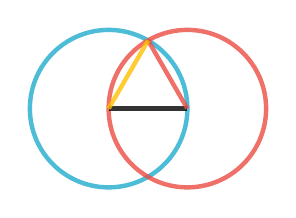
\begin{tikzpicture}[scale=1,opacity=0.8]
			\coordinate (A) at (0,0);
			\coordinate (B) at (1,0);
			\draw[name path=C1,blue,ultra thick] (A) circle (1cm);
			\draw[name path=C2,red,ultra thick] (B) circle (1cm);
			\path [name intersections={of=C1 and C2}];
			\coordinate (C) at (intersection-1);
			
			\draw[ultra thick] (A) -- (B); 
			\draw[ultra thick,red] (B) -- (C);
			\draw[ultra thick,yellow] (C) -- (A);
			\end{tikzpicture}
	%			text
%		\end{cutout}
	\end{prop}

	
	\begin{proof}
		Describe 
			
\begin{tikzpicture}[scale=0.5,opacity=0.8,baseline=-0.5ex]
			\coordinate (A) at (0,0);
			\coordinate (B) at (1,0);
			\draw[name path=C1,blue,ultra thick] (A) circle (1cm);
			\draw[ultra thick] (A) -- (B); 
			\end{tikzpicture}
		 and 
	 		
\begin{tikzpicture}[scale=0.5,opacity=0.8,baseline=-0.5ex]
	 		\coordinate (A) at (0,0);
	 		\coordinate (B) at (1,0);
	 		\draw[name path=C2,red,ultra thick] (B) circle (1cm);
	 		\draw[ultra thick] (A) -- (B); 
	 		\end{tikzpicture}
		 (\ref{post3}); draw \tikz[baseline=-0.5ex]\draw[yellow,ultra thick] (0,0) -- (1,0); and \tikz[baseline=-0.5ex]\draw[red,ultra thick] (0,0) -- (1,0); (\ref{post1}). then will 
	 	 		
\begin{tikzpicture}[baseline=-0.5ex,scale=0.5,opacity=0.8]
	 	 		\coordinate (A) at (0,0);
	 	 		\clip (-0.1,-0.1) rectangle (1.1,1.1);
	 	 		\coordinate (B) at (1,0);
	 	 		\path[name path=C1,blue,ultra thick] (A) circle (1cm);
	 	 		\path[name path=C2,red,ultra thick] (B) circle (1cm);
	 	 		\path [name intersections={of=C1 and C2}];
	 	 		\coordinate (C) at (intersection-1);
	 	 		\draw[ultra thick] (A) -- (B); 
	 	 		\draw[ultra thick,red] (B) -- (C);
	 	 		\draw[ultra thick,yellow] (C) -- (A);
	 	 		\end{tikzpicture}
		be equilateral. 
		\begin{align*}
			\text{For }  \tikz[baseline=-0.5ex]\draw[black,ultra thick] (0,0) -- (1,0); &= \tikz[baseline=-0.5ex]\draw[yellow,ultra thick] (0,0) -- (1,0);  (\text{ \ref{def15}})\\
			\text{and  }\tikz[baseline=-0.5ex]\draw[black,ultra thick] (0,0) -- (1,0); &= \tikz[baseline=-0.5ex]\draw[red,ultra thick] (0,0) -- (1,0); \text{ (\ref{def15})} \\
			\therefore \tikz[baseline=-0.5ex]\draw[yellow,ultra thick] (0,0) -- (1,0); &= \tikz[baseline=-0.5ex]\draw[red,ultra thick] (0,0) -- (1,0); \text{ (\ref{ax1})} 
		\end{align*}
	\end{proof}

		\clearpage
		\subsection{Proposition \the\numexpr \theprop + 1}
		
	\begin{prop}[Problem]
		\label{prop2}
		From a given point (
\begin{tikzpicture} [baseline=-0.5ex] \draw[red,ultra thick] (0,0) -- (0.6cm,0); \draw[blue,ultra thick] (0.6cm,0) -- (1cm,0);\end{tikzpicture}), 
			to draw a straight line equal to a given finite straight line (\tikzhline[black]{1cm}). % (\hline[black])	
	\end{prop}
	\begin{proof}
		Draw \tikzhline[densely dashed]{1cm} (\ref{post1}), describe 
		
\begin{tikzpicture}[scale=0.45,baseline=0.5ex]
			\draw[ultra thick,red] (0,0) -- (60:1) -- (1,0);
			\draw[ultra thick,densely dashed] (1,0) -- (0,0);
		\end{tikzpicture}
		(pr. 1.), produce \tikzhline[red]{0.7cm} (\ref{post2}), describe 
		
\begin{tikzpicture}[scale=0.4,baseline=-0.5ex]
			\draw[ultra thick] (0,0) -- (-1,0);
			\draw[blue,ultra thick] (0,0) circle (1cm);
		\end{tikzpicture}
		(\ref{post3}), and 
		
\begin{tikzpicture}[scale=0.4,baseline=-0.5ex]
			\draw[ultra thick,red] (0,0) -- (-60:0.4);
			\draw[ultra thick,yellow] (-60:0.4) -- (-60:1);
			\draw[ultra thick,red] (0,0) circle (1cm);
		\end{tikzpicture}

		(\ref{post3}); produce \tikzhline[red]{1cm} (\ref{post2}), then \tikzhline[blue]{1cm} is the line required. 
		For $
\begin{tikzpicture} [baseline=-0.5ex] \draw[yellow,ultra thick] (0,0) -- (0.6cm,0); \draw[red,ultra thick] (0.6cm,0) -- (1cm,0);\end{tikzpicture} = 
			
\begin{tikzpicture} [baseline=-0.5ex] \draw[red,ultra thick] (0,0) -- (0.4cm,0); \draw[blue,ultra thick] (0.4cm,0) -- (1cm,0);\end{tikzpicture}$
				(\ref{def15}), and $\tikzhline[red]{0.7cm} = \tikzhline[red]{0.7cm}$ (const.),
		$\therefore \tikzhline[yellow]{1cm} = \tikzhline[blue]{1cm}$ (\ref{ax3}), but (\ref{def15}) $\tikzhline[black]{1cm} = \tikzhline[yellow]{1cm} = \tikzhline[blue]{1cm}$;
		$\therefore \tikzhline[blue]{1cm}$ drawn from the given point 
		(
\begin{tikzpicture} [baseline=-0.5ex] \draw[red,ultra thick] (0,0) -- (0.4cm,0); \draw[blue,ultra thick] (0.4cm,0) -- (1cm,0);\end{tikzpicture}), 
			is equal the given line \tikzhline{1cm}.
		
	\end{proof}


		\clearpage
		\subsection{Proposition \the\numexpr \theprop + 1}
			\pagestyle{euclidprob}
    \begin{figure}[h]
        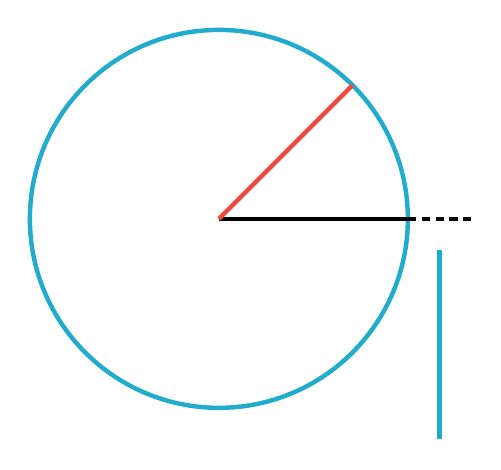
\begin{tikzpicture}[scale=0.8]
            \draw[ultra thick,blue] (0,0) circle (3cm);
            \draw[ultra thick,black] (0,0) -- (3,0);
            \draw[ultra thick,red] (0,0) -- (45:3cm);
            \draw[ultra thick,densely dashed] (3,0) -- (4,0);
            \draw[ultra thick,blue] (3.5,-0.5) -- (3.5,-3.5);
        \end{tikzpicture}
    \end{figure}

    \begin{prop}{\lettrine[lines=2]{F}rom}
		the greater (
\begin{tikzpicture} 
			\draw[ultra thick] (0,0) -- (0.9cm,0);
			\draw[densely dashed,ultra thick] (0.9cm,0) -- (1.5cm,0);
		\end{tikzpicture}
			) of two straight lines , to cut a part off equal to the less (\tikzhline[blue]{0.9cm}).\par

	\end{prop}
	\begin{proof}
		Draw $\tikzhline[red]{1cm} = \tikzhline[blue]{1cm}$ (\refprop{2}); 
        describe 
        
\begin{tikzpicture}[scale=0.5]
            \draw[ultra thick,red] (0,0) -- (45:1.15cm);
            \draw[ultra thick,blue] (0,0) circle (1cm);
        \end{tikzpicture}
        (\refpost{3}), then $\tikzhline[blue]{0.9cm} \equals \tikzhline[black]{0.9cm}.$
        \begin{align*}
            \text{For } \tikzhline[red]{0.9cm} &\equals \tikzhline[black]{0.9cm} \text{ (\refdef{15})}, \\
            \text{and } \tikzhline[blue]{0.9cm} &\equals \tikzhline[red]{0.9cm} \text{ (const.)}; \\
            \therefore\, \tikzhline[blue]{0.9cm} &\equals \tikzhline[black]{0.9cm} \text{ (\refax{1})}. 
        \end{align*}
	\end{proof}

		\clearpage
		\subsection{Proposition \the\numexpr \theprop + 1}
			\pagestyle{euclidthm}
    \begin{figure}[h]
      \begin{subfigure}{0.35\textwidth}
        \begin{tikzpicture}[scale=0.8]
            \coordinate (C) at (0,0);
            \coordinate (B) at (4,1);
            \coordinate (A) at (3,4);
            \tikzsectorabc[fill=red]{(A)}{(B)}{(C)}{0.2}
            \tikzsectorabc[fill=blue]{(B)}{(C)}{(A)}{0.2}
            \tikzsectorabc[fill=yellow]{(C)}{(A)}{(B)}{0.2}
            \tikztriangle[blue][black][red]{(A)}{(B)}{(C)}
        \end{tikzpicture}
      \end{subfigure}
      \begin{subfigure}{0.35\textwidth}
        \begin{tikzpicture}[scale=0.8]
            \coordinate (C) at (0,0);
            \coordinate (B) at (4,1);
            \coordinate (A) at (3,4);
            \tikzsectorabc[fill=red]{(A)}{(B)}{(C)}{0.2}
            \tikzsectorabc[fill=blue]{(B)}{(C)}{(A)}{0.2}
            \tikzsectorabc[fill=yellow]{(C)}{(A)}{(B)}{0.2}
            \tikztriangle[blue][black][red]{(A)}{(B)}{(C)}
        \end{tikzpicture}
      \end{subfigure}
    \end{figure}

    \def\cab{
        \begin{tikzpicture}[scale=0.8]
            \coordinate (C) at (0,0);
            \coordinate (B) at (4,1);
            \coordinate (A) at (3,4);
            \tikzsectorabc[fill=yellow]{(C)}{(A)}{(B)}{0.2}
        \end{tikzpicture}
    }
    \def\abc{
        \begin{tikzpicture}[scale=0.8]
            \coordinate (C) at (0,0);
            \coordinate (B) at (4,1);
            \coordinate (A) at (3,4);
            \tikzsectorabc[fill=red]{(A)}{(B)}{(C)}{0.2}
        \end{tikzpicture}
    }
    \def\bca{
        \begin{tikzpicture}[scale=0.8]
            \coordinate (C) at (0,0);
            \coordinate (B) at (4,1);
            \coordinate (A) at (3,4);
            \tikzsectorabc[fill=blue]{(B)}{(C)}{(A)}{0.2}
        \end{tikzpicture}
    }
    \def\ab{\tikzhline[red]{0.5cm}}
    \def\bc{\tikzhline[blue]{0.5cm}}
    \def\ac{\tikzhline[black]{0.5cm}}
    \begin{prop}{\lettrine[lines=2]{I}f}
      two triangles have two sides of the one respectively equal to two 
      sides of the other, (\ac to \ac and \ab to \ab) and the angles (\cab 
      and \cab) contained by those equals sides also equal; then their 
      bases or their sides (\bc and \bc) are also equal: and the remaining 
      and their remaining angles opposite to equal sides are respectively 
      equal ($\bca \equals \bca$ and  $\abc \equals \abc$): and the triangles are equal in 
      every respect.
  \end{prop}
	\begin{proof}
    Let the two triangles be conceived, to be so placed, that the vertex 
    of the one of the equal angles, \cab or \cab ; shall fall upon that of 
    the other, and \ac to coincide with \ac, then will \ac coincide with \ac 
    is applied: consequently \bc will coincide with \bc, or two straight 
    lines will enclose a space, which is impossible (\refax{10}), therefore 
    $\bc = \bc$, 
	\end{proof}

		\clearpage
		\subsection{Proposition \the\numexpr \theprop + 1}
			\pagestyle{euclidthm}
    \newcommand{\coordspec}{
      \coordinate (A) at (0,5)    ;
      \coordinate (B) at (-3.5,-2);
      \coordinate (C) at (3.5,-2) ;
      \path (A) -- (B) node[coordinate,pos=0.6] (D) {D};
      \path (A) -- (C) node[coordinate,pos=0.6] (E) {E};
      \pgfresetboundingbox
    }
    \begin{figure}[h]
        \begin{tikzpicture}[scale=0.8]
            \coordspec
            \tikzsectorabc[fill=black]{(B)}{(A)}{(C)}{1cm}
            \tikzsectorabc[fill=blue]{(E)}{(D)}{(A)}{1cm}
            \tikzsectorabc[fill=blue]{(A)}{(E)}{(D)}{1cm}
            \tikzsectorabc[fill=yellow]{(C)}{(D)}{(E)}{1cm}
            \tikzsectorabc[fill=yellow]{(D)}{(E)}{(B)}{1cm}
            \tikzsectorabc[fill=red]{(E)}{(B)}{(A)}{1cm}
            \tikzsectorabc[fill=red]{(A)}{(C)}{(D)}{1cm}
            \tikztriangle[yellow][blue][red]{(A)}{(B)}{(E)}
            \tikztriangle[yellow][blue][red]{(A)}{(C)}{(D)}
            \tikztriangle[red][black][red]{(A)}{(D)}{(E)}
        \end{tikzpicture}
    \end{figure}
    \newcommand{\ADE}{
        \begin{tikzpicture}[scale=0.1]
            \coordspec
            \tikztriangle[red][black][red]{(A)}{(D)}{(E)}
            \pgfresetboundingbox
            \path (A) -- (D) -- (E) -- cycle;
        \end{tikzpicture}
    }
    \newcommand{\ABE}{
        \begin{tikzpicture}[scale=0.2,baseline=-0.5cm]
            \coordspec
            \tikzsectorabc[fill=black]{(B)}{(A)}{(C)}{0.3cm}
            \tikztriangle[yellow][blue][red]{(A)}{(B)}{(E)}
            \pgfresetboundingbox
            \path (A) -- (B) -- (E) -- cycle;
%            \draw[red,ultra thick] (E) -- (A) -- (D);
        \end{tikzpicture}
    }
    \newcommand{\ACD}{
        \begin{tikzpicture}[scale=0.2,baseline=-0.5cm]
            \coordspec
            \tikzsectorabc[fill=black]{(B)}{(A)}{(C)}{0.3cm}
            \tikztriangle[yellow][blue][red]{(A)}{(C)}{(D)}
            \pgfresetboundingbox
            \path (A) -- (C) -- (D) -- cycle;
%            \draw[red,ultra thick] (E) -- (A) -- (D);
        \end{tikzpicture}
    }
    \newcommand{\DEB}{
        \begin{tikzpicture}[scale=0.2]
            \coordspec
            \tikztriangle[black][blue][yellow]{(D)}{(E)}{(B)}
            \pgfresetboundingbox
            \path (D) -- (E) -- (B) -- cycle;
        \end{tikzpicture}
    }
    \newcommand{\EDC}{
        \begin{tikzpicture}[scale=0.2]
            \coordspec
            \tikztriangle[black][blue][yellow]{(E)}{(D)}{(C)}
            \pgfresetboundingbox
            \path (E) -- (D) -- (C) -- cycle;
        \end{tikzpicture}
    }
    \newcommand{\bac}{
      \begin{tikzpicture}
        \coordspec
        \tikzsectorabc[fill=black]{(B)}{(A)}{(C)}{0.5cm}
      \end{tikzpicture}
    }
    \newcommand{\abe}{
      \begin{tikzpicture}
        \coordspec
        \tikzsectorabc[fill=red]{(E)}{(B)}{(A)}{0.5cm}
      \end{tikzpicture}
    }
    \newcommand{\acd}{
      \begin{tikzpicture}
        \coordspec
        \tikzsectorabc[fill=red]{(A)}{(C)}{(D)}{0.5cm}
      \end{tikzpicture}
    }
    \newcommand{\adc}{
      \begin{tikzpicture}
        \coordspec
        \tikzsectorabc[fill=blue]{(E)}{(D)}{(A)}{0.5cm}
        \tikzsectorabc[fill=yellow]{(C)}{(D)}{(E)}{0.5cm}
      \end{tikzpicture}
    }
    \newcommand{\aeb}{
      \begin{tikzpicture}
        \coordspec
        \tikzsectorabc[fill=blue]{(A)}{(E)}{(D)}{0.5cm}
        \tikzsectorabc[fill=yellow]{(D)}{(E)}{(B)}{0.5cm}
      \end{tikzpicture}
    }
    \newcommand{\ade}{
      \begin{tikzpicture}
        \coordspec
        \tikzsectorabc[fill=blue]{(E)}{(D)}{(A)}{0.5cm}
      \end{tikzpicture}
    }
    \newcommand{\aed}{
      \begin{tikzpicture}
        \coordspec
        \tikzsectorabc[fill=blue]{(A)}{(E)}{(D)}{0.5cm}
      \end{tikzpicture}
    }
    \newcommand{\dec}{
      \begin{tikzpicture}
        \coordspec
        \tikzsectorabc[fill=white,draw=black]{(B)}{(E)}{(C)}{0.5cm}
        \draw (E) -- ($(E)!0.5cm!(C)$);
        \tikzsectorabc[fill=yellow]{(D)}{(E)}{(B)}{0.5cm}
      \end{tikzpicture}
    }
    \newcommand{\edc}{
      \begin{tikzpicture}
        \coordspec
        \tikzsectorabc[fill=yellow]{(C)}{(D)}{(E)}{0.5cm}
      \end{tikzpicture}
    }
    \newcommand{\deb}{
      \begin{tikzpicture}
        \coordspec
        \tikzsectorabc[fill=yellow]{(D)}{(E)}{(B)}{0.5cm}
      \end{tikzpicture}
    }
    \newcommand{\edb}{
      \begin{tikzpicture}
        \coordspec
        \tikzsectorabc[fill=white,draw=black]{(B)}{(D)}{(C)}{0.5cm}
        \draw (D) -- ($(D)!0.5cm!(B)$);
        \tikzsectorabc[fill=yellow]{(C)}{(D)}{(E)}{0.5cm}
      \end{tikzpicture}
    }
    \def\ab{
      \tikzhline[red]{0.5cm}\tikzhline[yellow]{0.5cm}
    }
    \def\ac{
      \tikzhline[red]{0.5cm}\tikzhline[yellow]{0.5cm}
    }
    \newcommand{\ad}{
      \tikzhline[red]{1cm}
    }
    \def\ae{
      \tikzhline[red]{1cm}
    }
    \newcommand{\db}{
      \tikzhline[yellow]{1cm}
    }
    \newcommand{\dc}{
      \tikzhline[blue]{1cm}
    }
    \newcommand{\eb}{
      \tikzhline[blue]{1cm}
    }
    \newcommand{\ec}{
      \tikzhline[yellow]{1cm}
    }

    

    \begin{prop}{\lettrine[lines=2]{I}n}
        any isosceles triangle \ADE if the equal sides be produced, the external angles at the base are equal, and the internal angles at the base are also equal. 
	\end{prop}
	\begin{proof}
        Produce \ad, and \ae, (\refpost{2}), take $\db \equals \ec$, (\refprop{3}); draw \dc and \eb. 

        Then in \ABE and \ACD we have, $\ab \equals \ac$ (const.), \bac common to both, and $\ad \equals \ae$ (hyp.) $\therefore \adc \equals \aeb$, $\dc \equals \eb$ and $\abe \equals \acd$ (\refprop{4}). Again in \DEB and \EDC we have $\db \equals \ec$, $\abe \equals \acd$ and $\dc \equals \eb$, \therefore\ $\edb \equals \dec$ and $\edc \equals \deb$  (\refprop{4}) but $\adc \equals \aeb$, $\therefore \ade \equals \aed$ (\refax{3}). 
	\end{proof}

		\clearpage


\end{document}